% \documentclass[table]{beamer}
\documentclass[table,handout]{beamer}
\setbeameroption{show notes}
% \setbeameroption{hide notes}
% \setbeameroption{show only notes}
\usepackage{varwidth}

\newif\ifhide
\newif\ifpost
\newif\ifhideclicker

% \hidetrue
% \hideclickertrue
% \posttrue

\newcommand{\whiteout}[1]{\textcolor{white}{#1}}
% \newcommand{\whiteoutbox}[1]{\fcolorbox{white}{white}{\parbox{\dimexpr \linewidth-2\fboxsep-2\fboxrule}{\whiteout{#1}}}}
% \newcommand{\notebox}[1]{\fcolorbox{blue}{white}{\parbox{\dimexpr \linewidth-2\fboxsep-2\fboxrule}{#1}}}
\newcommand{\whiteoutbox}[1]{\fcolorbox{white}{white}{\parbox{\linewidth}{\whiteout{#1}}}}
\newcommand{\notebox}[1]{\fcolorbox{blue}{white}{\parbox{\linewidth}{#1}}}
\newcommand{\blankbox}[1]{\phantom{\varwidth{\linewidth}\whiteoutbox{#1}\endvarwidth}}
\newcommand{\blank}[1]{\phantom{\varwidth{\linewidth}#1\endvarwidth}}

\ifhide%
    \newcommand{\hmask}[1]{\blank{#1}}%
\else%
    \newcommand{\hmask}[1]{#1}%
\fi

\ifhide%
    \newcommand{\wout}[1]{\whiteout{#1}}%
\else%
    \newcommand{\wout}[1]{#1}%
\fi

\ifhide%
    \newcommand{\hignore}[1]{}%
\else%
    \newcommand{\hignore}[1]{#1}%
\fi

\ifpost%
    \newcommand{\nopost}[1]{}%
\else%
    \newcommand{\nopost}[1]{#1}%
\fi

\ifhideclicker%
    \newcommand{\clickerslide}[1]{\stepcounter{clickerQuestionCounter}%
        \begin{frame}[t]
            \textcolor{blue}{Q \arabic{clickerQuestionCounter}:}
        \end{frame}}
\else%
    \newcommand{\clickerslide}[1]{#1}%
\fi

\ifhide%
    \newcommand{\hidebox}[1]{\blank{#1}}%
\else%
    \newcommand{\hidebox}[1]{\notebox{#1}}%
\fi

\ifhide%
    \newcommand{\wbox}[1]{\whiteoutbox{#1}}%
\else%
    \newcommand{\wbox}[1]{\notebox{#1}}%
\fi

\ifhide%
    \newcommand{\nbox}[1]{\blankbox{#1}}%
\else%
    \newcommand{\nbox}[1]{\notebox{#1}}%
\fi

\ifhideclicker%
    \newcommand{\clickeranswer}[1]{#1}%
\else%
    \ifhide%
        \newcommand{\clickeranswer}[1]{#1}%
    \else%
        \newcommand{\clickeranswer}[1]{\textbf{\textcolor{blue}{#1}}}%
    \fi
\fi

\usepackage{beamerthemesplit}
% \usetheme{boxes}
\usetheme{Malmoe}
\usecolortheme{seahorse}
% \usecolortheme{seagull}
\usepackage{ifthen}
\usepackage{xspace}
\usepackage{multirow}
\usepackage{multicol}
\usepackage{booktabs}
\usepackage{xcolor}
\usepackage{wasysym}
\usepackage{comment}
\usepackage{hyperref}
\hypersetup{pdfborder={0 0 0}, colorlinks=true, urlcolor=blue, linkcolor=blue, citecolor=blue}
\usepackage{changepage}
\usepackage[compatibility=false]{caption}
\captionsetup[figure]{font=scriptsize, labelformat=empty, textformat=simple, justification=centering, skip=2pt}
\usepackage{tikz}
\usetikzlibrary{trees,calc,backgrounds}

\usepackage[bibstyle=joaks-slides,maxcitenames=3,mincitenames=1,backend=biber]{biblatex}

\newrobustcmd*{\shortfullcite}{\AtNextCite{\renewbibmacro{title}{}\renewbibmacro{in:}{}\renewbibmacro{number}{}}\fullcite}

\newrobustcmd*{\footlessfullcite}{\AtNextCite{\renewbibmacro{title}{}\renewbibmacro{in:}{}}\footfullcite}

% Make all footnotes smaller
% \renewcommand{\footnotesize}{\scriptsize}

\definecolor{myGray}{gray}{0.9}
\colorlet{rowred}{red!30!white}

\setbeamertemplate{blocks}[rounded][shadow=true]

\setbeamercolor{defaultcolor}{bg=structure!30!normal text.bg,fg=black}
\setbeamercolor{block body}{bg=structure!30!normal text.bg,fg=black}
\setbeamercolor{block title}{bg=structure!50!normal text.bg,fg=black}

\newenvironment<>{varblock}[2][\textwidth]{%
  \setlength{\textwidth}{#1}
  \begin{actionenv}#3%
    \def\insertblocktitle{#2}%
    \par%
    \usebeamertemplate{block begin}}
  {\par%
    \usebeamertemplate{block end}%
  \end{actionenv}}

\newenvironment{displaybox}[1][\textwidth]
{
    \centerline\bgroup\hfill
    \begin{beamerboxesrounded}[lower=defaultcolor,shadow=true,width=#1]{}
}
{
    \end{beamerboxesrounded}\hfill\egroup
}

\newenvironment{onlinebox}[1][4cm]
{
    \newbox\mybox
    \newdimen\myboxht
    \setbox\mybox\hbox\bgroup%
        \begin{beamerboxesrounded}[lower=defaultcolor,shadow=true,width=#1]{}
    \centering
}
{
    \end{beamerboxesrounded}\egroup
    \myboxht\ht\mybox
    \raisebox{-0.25\myboxht}{\usebox\mybox}\hspace{2pt}
}

\newenvironment{mydescription}{
    \begin{description}
        \setlength{\leftskip}{-1.5cm}}
    {\end{description}}

\newenvironment{myitemize}{
    \begin{itemize}
        \setlength{\leftskip}{-.3cm}}
    {\end{itemize}}

% footnote without a marker
\newcommand\barefootnote[1]{%
  \begingroup
  \renewcommand\thefootnote{}\footnote{#1}%
  \addtocounter{footnote}{-1}%
  \endgroup
}

% define formatting for footer
\newcommand{\myfootline}{%
    {\it
    \insertshorttitle
    \hspace*{\fill} 
    \insertshortauthor, \insertshortinstitute
    % \ifx\insertsubtitle\@empty\else, \insertshortsubtitle\fi
    \hspace*{\fill}
    \insertframenumber/\inserttotalframenumber}}

% set up footer
\setbeamertemplate{footline}{%
    \usebeamerfont{structure}
    \begin{beamercolorbox}[wd=\paperwidth,ht=2.25ex,dp=1ex]{frametitle}%
        % \Tiny\hspace*{4mm}\myfootline\hspace{4mm}
        \tiny\hspace*{4mm}\myfootline\hspace{4mm}
    \end{beamercolorbox}}

% remove navigation bar
\beamertemplatenavigationsymbolsempty

\makeatletter
    \newenvironment{noheadline}{
        \setbeamertemplate{headline}[default]
        \def\beamer@entrycode{\vspace*{-\headheight}}
    }{}
\makeatother

\newcounter{clickerQuestionCounter}
\ifhideclicker%
\newenvironment{clickerquestion}
{ \stepcounter{clickerQuestionCounter}
  \begin{enumerate}[Q \arabic{clickerQuestionCounter}:]\color{white} }
{ \end{enumerate} }
\else%
\newenvironment{clickerquestion}
{ \stepcounter{clickerQuestionCounter}
  \begin{enumerate}[Q \arabic{clickerQuestionCounter}:] }
{ \end{enumerate} }
\fi

\ifhideclicker%
\newenvironment{clickeroptions}
{ \begin{enumerate}[\begingroup\color{white} 1)\endgroup]\color{white} }
{ \end{enumerate} }
\else%
\newenvironment{clickeroptions}
{ \begin{enumerate}[\begingroup\color{red} 1)\endgroup] }
{ \end{enumerate} }
\fi


\tikzstyle{centered} = [align=center, text centered, font=\sffamily\bfseries]
\tikzstyle{skip} = [centered, inner sep=0pt, fill]
\tikzstyle{empty} = [centered, inner sep=0pt]
\tikzstyle{inode} = [centered, circle, minimum width=4pt, fill=black, inner sep=0pt]
\tikzstyle{tnode} = [centered, circle, inner sep=1pt]
\tikzset{
  % edge styles
  level distance=10mm,
  mate/.style={edge from parent/.style={draw,distance=3pt}},
  mleft/.style={grow=left, level distance=10mm, edge from parent path={(\tikzparentnode.west)--(\tikzchildnode.east)}},
  mright/.style={grow=right, level distance=10mm, edge from parent path={(\tikzparentnode.east)--(\tikzchildnode.west)}},
  % node styles
  male/.style={rectangle,minimum size=4mm,fill=gray!80},
  female/.style={circle,minimum size=4mm,fill=gray!80},
  amale/.style={male,fill=red},
  afemale/.style={female,fill=red},
}

\newcommand{\highlight}[1]{\textcolor{violet}{\textit{\textbf{#1}}}}
\newcommand{\super}[1]{\ensuremath{^{\textrm{\sffamily #1}}}}
\newcommand{\sub}[1]{\ensuremath{_{\textrm{\sffamily #1}}}}
\newcommand{\dC}{\ensuremath{^\circ{\textrm{C}}}}
\newcommand{\tb}{\hspace{2em}}
\providecommand{\e}[1]{\ensuremath{\times 10^{#1}}}
\newcommand{\myHangIndent}{\hangindent=5mm}

\newcommand{\spp}[1]{\textit{#1}}

\newcommand\mybullet{\leavevmode%
\usebeamertemplate{itemize item}\hspace{.5em}}

\makeatletter
\newcommand*{\rom}[1]{\expandafter\@slowromancap\romannumeral #1@}
\makeatother

\newcommand{\blankslide}{{\setbeamercolor{background canvas}{bg=black}
\setbeamercolor{whitetext}{fg=white}
\begin{frame}<handout:0>[plain]
\end{frame}}}

\newcommand{\whiteslide}{
\begin{frame}<handout:0>[plain]
\end{frame}}

\newcommand{\f}[1]{\ensuremath{F_{#1}}}
\newcommand{\x}[1]{X\ensuremath{^{#1}}}
\newcommand{\y}[1]{Y\ensuremath{^{#1}}}

% Population growth macros
\newcommand{\popsize}[1]{\ensuremath{N_{#1}}}
\newcommand{\popgrowthratediscrete}[1]{\ensuremath{\lambda_{#1}}}
\newcommand{\popgrowthrate}[1]{\ensuremath{r_{#1}}}
\newcommand{\ptime}{\ensuremath{t}\xspace}

\tikzset{hide on/.code={\only<#1>{\color{white}}}}
\tikzset{
    invisible/.style={opacity=0},
    visible on/.style={alt={#1{}{invisible}}},
    alt/.code args={<#1>#2#3}{%
        \alt<#1>{\pgfkeysalso{#2}}{\pgfkeysalso{#3}}
        % \pgfkeysalso doesn't change the path
    },
}

% \bibliography{../bib/references}
\bibliography{references}
\author[J.\ Oaks]{
    %Jamie R.\ Oaks\inst{1}
    Jamie R.\ Oaks
}
\institute[BIOL 180]{
    \inst{}%
        BIOL 180: Introductory Biology
}



\newcommand{\Y}{{\tikz\draw[black,fill=yellow] (0,0) circle (1ex);}\xspace}
\newcommand{\G}{{\tikz\draw[black,fill=green] (0,0) circle (1ex);}\xspace}

\title[Statistics]{Data Analysis and Statistics}
% \date{\today}
\date{April 20, 2015}

\begin{document}

\begin{noheadline}
\maketitle
\end{noheadline}

\nopost{
\begin{noheadline}
\begin{frame}[c]
    \vspace{-1.3cm}
    \begin{center} 
        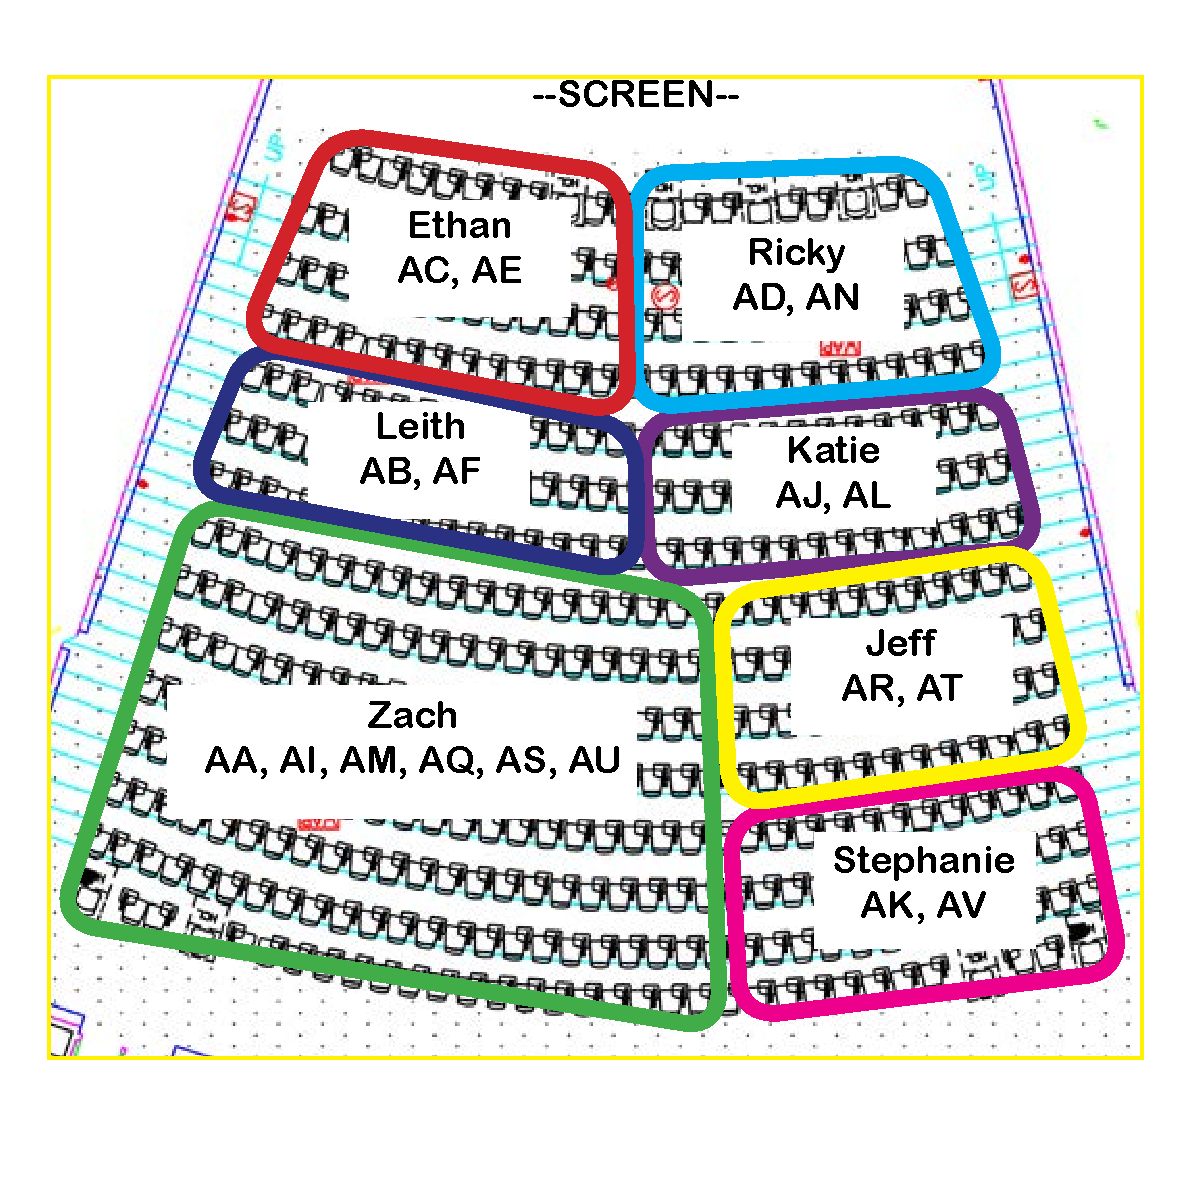
\includegraphics[height=1.3\textheight]{../images/seating-chart.pdf}
    \end{center}
\end{frame}
\end{noheadline}
}

\begin{noheadline}
\begin{frame}
\frametitle{Today's issues:}
\tableofcontents
\end{frame}
\end{noheadline}

\section{Basics of probability}

\clickerslide{
\begin{frame}
    \begin{clickerquestion}
        \item If I flip a fair coin and roll a fair 6-sided die, what is the
            probability that I get a heads and a 1 \textit{\textbf{OR}} a tails
            and a 6?
        \begin{clickeroptions}
            \item 1/12
            \item 1/144
            \item 4/9
            \item \clickeranswer{1/6}
            \item 0.25
        \end{clickeroptions}
    \end{clickerquestion}
\end{frame}
}

\clickerslide{
\begin{frame}
    \begin{clickerquestion}
        \item What is the probability of getting at least two heads in three
            flips of a fair coin?
        \begin{clickeroptions}
            \item \clickeranswer{0.5}
            \item 0.25
            \item 1/8
            \item 3/8
            \item 0.75
        \end{clickeroptions}
    \end{clickerquestion}
\end{frame}
}

\section{Frequentist inference: hypothesis testing}

\begin{frame}
    \begin{itemize}[<+->]
        \item We find a species of plant in which some individuals have yellow
            seeds and others have green seeds.
        \item This species of plant is closely related to the garden peas that
            Mendel used.
        \item Luckily enough, some plant breeders have already bred pure lines
            for each seed color.
        \item We cross individuals from yellow-seeded and green-seeded pure
            lines, and all of the \f{1} progeny have yellow seeds.
        \item The plant breeders tell us that when they cross \f{1}s with
            pure-line green-seeded individuals, they sometimes see more yellow
            seeds than they expect.
        \item The breeders hypothesize that heterozygotes produce more gametes
            with the yellow allele than the green allele.

    \end{itemize}
\end{frame}

\clickerslide{
\begin{frame}
    \begin{clickerquestion}
        \item
            Based on Mendel's work, what is a good \highlight{null} hypothesis
            for how this trait is inherited?
        \begin{clickeroptions}
            \item Seed color is controlled by a single gene with two alleles
                that assort independently during meiosis.
            \item Seed color is controlled by a two genes that segregate during
                meiosis.
            \item Seed color is controlled by a two genes that assort
                independently during meiosis.
            \item \clickeranswer{Seed color is controlled by a single gene with
                    two alleles that segregate during meiosis.}
        \end{clickeroptions}
    \end{clickerquestion}
\end{frame}
}

\clickerslide{
\begin{frame}
    \begin{clickerquestion}
        \item
            If we cross an \f{1} male to a female from the green-seeded pure
            line, what ratio of yellow-seeded to green-seeded progeny do we
            expect to find if our null hypothesis is correct?
        \begin{clickeroptions}
            \item 3:1
            \item \clickeranswer{1:1}
            \item 1:3
            \item 9:3:3:1
        \end{clickeroptions}
    \end{clickerquestion}
\end{frame}
}

\begin{frame}
    \begin{itemize}
        \item<1-> We cross an \f{1} male to a female from the green-seeded pure
            line, and we get 3 yellow-seeded and 1 green-seeded offspring

            \vspace{0.5cm}
        \item<2-> Our null hypothesis predicted a 1:1 ratio, and we found a 3:1
            ratio.  What should we do? Is the null wrong?

            \vspace{0.5cm}
        \item<3-> How likely were we to get our results due to chance?
    \end{itemize}
\end{frame}

\begin{frame}
    We need to figure out the probability of outcomes under the null
    hypothesis.

    \vspace{1cm}
    Was our null hypothesis a good null hypothesis?
    \nbox{Yes---It makes precise predictions, which allow us to calculate
        the probability of all possible outcomes of our experiment.}
\end{frame}

\begin{frame}
    \frametitle{All possible results}
    \begin{columns}
        \column{0.33\textwidth}
        \Y,\Y,\Y,\Y

        \vspace{0.5cm}
        \Y,\Y,\Y,\G \\
        \Y,\Y,\G,\Y \\
        \Y,\G,\Y,\Y \\
        \G,\Y,\Y,\Y

        \column{0.33\textwidth}
        \Y,\Y,\G,\G \\
        \Y,\G,\Y,\G \\
        \Y,\G,\G,\Y \\
        \G,\Y,\G,\Y \\
        \G,\G,\Y,\Y \\
        \G,\Y,\Y,\G

        \column{0.33\textwidth}
        \Y,\G,\G,\G \\
        \G,\Y,\G,\G \\
        \G,\G,\Y,\G \\
        \G,\G,\G,\Y

        \vspace{0.5cm}
        \G,\G,\G,\G
    \end{columns}

    \vspace{1cm}
    \uncover<2->{Which results are as ``weird'' as the results we found (3
        yellow: 1 green)?  What's the total probability of these unexpected
        results?}

\end{frame}

\clickerslide{
\begin{frame}
    \begin{clickerquestion}
        \item What does the probability 0.625 (10/16) represent regarding our
            experiment?
        \begin{clickeroptions}
            \item The probability of getting results as weird as what we
                actually observed, assuming the null hypothesis is incorrect.
            \item The probability of the null hypothesis.
            \item \clickeranswer{The probability of getting results as weird as
                    what we actually observed, under the null hypothesis (i.e.,
                    assuming the null hypothesis is correct).}
            \item The probability that the null hypothesis is incorrect.
        \end{clickeroptions}
    \end{clickerquestion}

    \vspace{1cm}
    What do we call this probability?

    \nbox{The p-value}
\end{frame}
}

\begin{frame}
    \frametitle{All possible results}
    \begin{columns}
        \column{0.33\textwidth}
        \Y,\Y,\Y,\Y

        \vspace{0.5cm}
        \Y,\Y,\Y,\G \\
        \Y,\Y,\G,\Y \\
        \Y,\G,\Y,\Y \\
        \G,\Y,\Y,\Y

        \column{0.33\textwidth}
        \Y,\Y,\G,\G \\
        \Y,\G,\Y,\G \\
        \Y,\G,\G,\Y \\
        \G,\Y,\G,\Y \\
        \G,\G,\Y,\Y \\
        \G,\Y,\Y,\G

        \column{0.33\textwidth}
        \Y,\G,\G,\G \\
        \G,\Y,\G,\G \\
        \G,\G,\Y,\G \\
        \G,\G,\G,\Y

        \vspace{0.5cm}
        \G,\G,\G,\G
    \end{columns}

    \vspace{1cm}
    \uncover<1->{If we consider a p-value of 0.05 or less as significant, what
        was wrong with our experiment?}

    \nbox{Our sample size is too small to ever get a significant result}

    \uncover<1->{What can we do?}

    \nbox{Increase our sample size or perform more replicates.}

\end{frame}

\clickerslide{
\begin{frame}
    \begin{clickerquestion}
        \item We repeat our experiment and get the same ratio (3 yellow: 1
            green), but this time we sampled 20 progeny. What will happen to
            our p-value relative to our previous result?
        \begin{clickeroptions}
            \item \clickeranswer{It will decrease.}
            \item It will stay the same.
            \item It will increase.
            \item It will prove the null hypothesis is wrong.
        \end{clickeroptions}
    \end{clickerquestion}
\end{frame}
}

\begin{frame}
    \uncover<1->{
        The probability of getting a result as weird as 15 yellow: 5 green,
        assuming the null hypothesis is correct, is 0.041.}

        \vspace{4mm}
    \uncover<1->{
        What do we do?
            \nbox{Given our results are so unlikely under the null hypothesis,
                we can assume it is not a good explanation of what is going on
                (we ``reject'' the null hypothesis).}}

        \vspace{0.3cm}
    \uncover<1->{
        What is the probability of the null hypothesis?
        \nbox{We don't know; in frequentist statistical tests, we can only make
            probability statements about the data (or summary statistics
            calculated from the data), \highlight{NOT} the hypotheses.}}
    \uncover<1->{
        What is the probability of our results under the ``alternative''
        hypothesis?
        \nbox{We don't know; statistical tests always test the null hypothesis.
            If we reject the null, we can often conclude our alternative
            hypothesis is a better explanation. However, we usually cannot
            quantify how well it explains the data.}}
\end{frame}

\begin{frame}[t]
    We were able to reject the null hypothesis of simple Mendelian
    inheritance. So, what now? \\

    \vspace{8mm}
    Our alternative hypothesis was that heterozygotes produce more gametes with
    the yellow allele than the green allele. \\

    \vspace{8mm}
    What is the next step? How do we continue to advance science? \\

    \nbox{We need to come up with a \highlight{mechanism} for the alternative
        hypothesis that allows us to make precise predictions about the data we
        should see if it is correct. This would make the alternative hypothesis
        into a good null hypothesis that we can test quantitatively.} 
\end{frame}

% \section{Bayesian inference teaser}

% \begin{frame}[t]
%     \begin{itemize}
%         \item<1->The proportion of people in the USA with HIV is 0.003 (3/1000). 
%         \item<2->The test for HIV is very accurate:
%             \begin{itemize}
%                 \item<3-> The probability of a positive test if a person has
%                     HIV is 0.998.
%                 \item<4-> The probability of a positive test if a person is
%                     healthy is 0.015.
%             \end{itemize}
%     \end{itemize}

% \end{frame}

% \begin{frame}[t]
%     \begin{itemize}
%         \item The proportion of people in the USA with HIV is 0.003 (3/1000). 
%         \item The test for HIV is very accurate:
%             \begin{itemize}
%                 \item The probability of a positive test if a person has
%                     HIV is 0.998.
%                 \item The probability of a positive test if a person is
%                     healthy is 0.015.
%             \end{itemize}
%     \end{itemize}

%     \begin{clickerquestion}
%         \item If we randomly sample someone from the population, test them, and
%             find a positive result, what is the probability this individual has
%             HIV?
%         \begin{clickeroptions}
%             \item 0.998
%             \item 0.985
%             \item \clickeranswer{0.167}
%             \item 0.881
%         \end{clickeroptions}
%     \end{clickerquestion}
% \end{frame}

\end{document}

